\documentclass[conference]{IEEEtran}
\IEEEoverridecommandlockouts
% The preceding line is only needed to identify funding in the first footnote. If that is unneeded, please comment it out.
\usepackage{cite}
\usepackage{amsmath,amssymb,amsfonts}
\usepackage{algorithmic}
\usepackage{graphicx}
\usepackage{textcomp}
\usepackage{xcolor}
\usepackage{float}


\bibliographystyle{IEEEtran}	
\def\BibTeX{{\rm B\kern-.05em{\sc i\kern-.025em b}\kern-.08em
T\kern-.1667em\lower.7ex\hbox{E}\kern-.125emX}}
\begin{document}

\title{Role of positive feedback in employee well-being working with an intelligent assistant in manufacturing\\
}

\author{\IEEEauthorblockN{Akshay Chikhalkar}
\IEEEauthorblockA{\textit{Department of Electrical Engineering and Computer Science} \\
\textit{Technical Hocschule Ostwestfalen-Lippe - University of Applied Sciences and Arts}\\
Lemgo, Germany \\
akshay.chikhalkar@stud.th-owl.de}

}

\maketitle

\begin{abstract}
	Employee well-being is a state of being comfortable, healthy, and happy, and organisations need to promote it to ensure success. Employee satisfaction in the retail sector increased by 11\% from January to December 2020, according to Glint's Employee Well-Being Report, but employee burnout in the manufacturing sector increased by 86\%. This suggests that employees in the manufacturing industry feel more stressed and overwhelmed than those in other industries. The manufacturing sector was still over 647,000 jobs short of its pre-pandemic levels, according to the October U.S. jobs report, showing that many workers are working with insufficient staff and an increased workload. This can lead to stress and burnout, negatively impacting employee well-being. This is due to the rise in constantly changing manufacturing technologies, required skills, and stress-related absenteeism and presenteeism, with workplace stress costing employers in the US nearly 200 billion dollars annually. Performance and employee well-being are strongly correlated. This relationship is consistent across all types of industries and is linked to workplace spirituality. The purpose of this study is to evaluate the effect of positive feedback on the well-being of the employee. An online survey was conducted on a wide demographic of people from all age groups to know their perspective on well-being. With the results, we aim to find the relationship between positive feedback and well-being by using statistical tests. 
\end{abstract}

\begin{IEEEkeywords}
	valence, well-being, positive feedback, positive affect
\end{IEEEkeywords}

\section{Introduction}
	The fourth industrial revolution was triggered by new and disruptive intelligence and information technologies. These new technologies enable ever-increasing efficiency in manufacturing through the use of Artificial Intelligence (AI), Augmented Reality (AR), Virtual Reality (VR), big data and analytics, blockchain, the cloud, advanced robotic assistance and simulation \cite{b1}.  Due to technological development, manufacturing processes are becoming increasingly complex, placing new kinds of demands on companies' management practises and processes, as well as on employees' competencies and skills \cite{b3}\cite{b4}\cite{b5}. Manufacturing companies that have a high level of technological competence can take advantage of and benefit from these technological developments, while companies with a lower level of competence are unlikely to be successful in competition \cite{b2}. This inevitably has an impact on the company and the health and well-being of its employees. As a result, attention must be paid to the employee's well-being. Psychological well-being (WB) encompasses the overall assessment of an employee’s life and affective state and is considered a key aspect of individual and group health \cite{b6}. Well-being is important for the sustainable growth of both employees and employers. Positive emotions, good feelings, motivation and recognition at work benefit employers by improving employee performance, engagement and retention. Studies have shown that intuitive task feedback plays an important role in influencing employee performance and well-being \cite{b7}. As Locke, Cartledge, and Knerr \cite{b8} argued, those who are satisfied with their past performance, will continue to perform at their current level, while those who are dissatisfied will change their performance. Based on this argument, feedback may contribute to enhancing task performance and well-being if the subject believes they are not progressing satisfactorily. However, the way positive feedback influences well-being is not yet fully understood.\\
	This paper sets out to address this knowledge gap. We investigated the effects of positive task feedback on the well-being (Positive Affect) of an employee. We focused on the Affect and Authentic Pride	especially the positive affect of well-being. It was hypothesized that positive task feedback would be associated with an increase in well-being. 

\section{Related Work}
	There are multiple studies based on well-being, one of which focused on well-being oriented human resource management practises and also supports the mediating role of well-being between Human Resource Management (HRM) and organisational performance \cite{b19}. The feedback and leadership fairness literature, in connecting fairness of leader feedback to Leader-Member Exchange (LMX) and important work-related outcomes, is more focused on supervisors' feedback \cite{b20}. Research aimed to evaluate job-related affective well-being, perceived supervisor support and positive feedback as contributing factors to the work engagement of lecturers in the context of two countries in South East Asia \cite{b21}. In addition, studies focused on well-being in different demographic, educational \& sports institutes but not on the manufacturing industry. The above studies say feedback is related to well-being but did not clarify the characteristics 
	of feedback. This paper aims to analyse the relationship between employee well-being and positive feedback working with an intelligent assistants (IA) in the manufacturing industry. 
	
\section{Well-being and Feedback}

	Employee well-being refers to the physical, mental, and social health and well-being of employees in an organization\cite{b22}. It encompasses a range of factors that can affect an employee’s overall sense of well-being and quality of life, including:\\
	Physical health: This includes factors such as access to health- care, safety in the workplace, and opportunities for physical activity.\cite{b24}\\
	Social health: This includes factors such as a sense of belonging, supportive relationships with colleagues, and opportunities for socialization.\cite{b24}\\
	Mental health: This includes factors such as stress management, work-life balance, and support for mental health issues.\cite{b25}\\
	Employee well-being is important because it can have a significant impact on an individual’s productivity, engagement, and overall job satisfaction.\\
	Feedback is a way of sharing information about a person’s performance or behaviour, intending to help them to improve or learn from the experience. Feedback can take many forms, including verbal or written comments, ratings, or evaluations. It can be provided by a supervisor, a peer, or a customer, and can be positive, negative, or neutral in nature. Effective feedback should be timely, specific, and respectful, and should focus on the behaviour or performance rather than the person\cite{b23}. It should also be balanced, providing both positive and constructive feedback to help the person understand their strengths and areas for improvement. 

\section[htbp]{Methodology}

	An online survey was conducted in English and German language. There were three questionnaires, two of them were for studying the feedback and one for the significance of well-being. The survey was distributed 40-40-20 by the study software, meaning that 40\% of participants received Questionnaire one, 40\% received Questionnaire two, and the remaining 20\% received Questionnaire three. Each questionnaire was created to capture the connection between the respondent and their perception of well-being. An instrument was designed to record multiple inputs from participants for each questionnaire accurately. In statistics, "instrumentation" refers to the equipment or methods used to quantify variables or other relevant factors throughout the data-gathering process \cite{b9}. In the feedback questionnaire, there were eight circumstances for each question that were displayed to participants along with screenshots, and participants’ responses were recorded on the Likert scale, which ranges from Strongly Agree to Strongly Disagree (1 to 7) as shown in \figurename{\ref{Likert Scale}}. The poll was done among participants who ranged in age from 18 to 84 and was equally divided among men and women. Also, it was equally divided between people under and over 50 years of age. On the data gathered from the survey, to check data reliability, we perform Unidimensional Reliability Test. Using an Independent Sample T-Test, the strength of the link between two variables was evaluated. A Spearman's Correlation Test is performed to strengthen results. In this paper, we seek to determine the connection between well-being and positive feedback. To compare the means of the two groups, we use an Independent Sample T-Test to determine whether there has been a significant difference in well-being and valence. 

	\begin{figure}[htbp]
	\centerline{
\includegraphics[width=95mm,scale=1]{likert_scale.jpeg}}
	\caption{Likert Scale}
	\label{Likert Scale}
	\end{figure}

	\subsection[htbp]{Data Analysis}
	
		A total of 500 replies were needed, however, the survey findings show that only 468 were submitted for all three questionaries. 379 of those responses are about task feedback. 60\% of the 379 responses came from men, while 40\% came from women. A little more than 86\% of participants were under 50, and 14\% were over. Participants came from 37 different nations in total, with 49\% of them being from Germany, 12\% from Gambia, 8\% from India and the remaining 31\% participants from other countries.. 40\% of participants obtained their undergraduate or graduate degrees, while 19\% finished their higher education. As a result, the majority of the study participants are well-educated. Nearly 52\% of respondents completed the survey in German, while 48\% did so in English. Participants in this study ranged in age from 17 to 84, with the majority falling between the ages of 18 and 40. \figurename{\ref{Descriptive statistics of the participants}} indicates the descriptive statistics of participants.\\ 
		
		\begin{figure}[htbp]
		\centerline{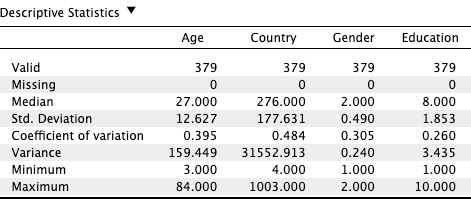
\includegraphics[width=88mm,scale=1]{Descriptive Statistics of participants.jpeg}}
		\caption{Descriptive statistics of the participants}
		\label{Descriptive statistics of the participants}
		\end{figure}
		We evaluate the results using JASP, a statistical analysis software programme created and maintained by the JASP team, a group of researchers and developers at the University of Amsterdam. The app is intended for researchers and students who are interested in conducting statistical analyses but may not have a strong background in statistics \cite{b10}. 
		
		\subsection{Data Preparation}
		
		To focus on the effect of positive feedback, we exclude data which was not related and only considered Questionary Set-1 for the analysis. The average was taken as well-being from 
		three variables (Satisfied, Successful, Confident) related to positive affect from an instrument to obtain a single value. Data were further filtered out to exclude control group records of independent variable valence as the control group does not contribute to the results. The analysis was performed on 164 samples, the data which resulted from the above steps. 
		
		\subsection[H]{Data Reliability}
		Data Reliability in statistics refers to the consistency of a measure when repeated multiple times \cite{b11}. It is an important factor for obtaining useful results from data collection methods \cite{b12}. Cronbach’s $\alpha$ is a measure used to assess the reliability of a set of scale or test items \cite{b13}. It is most commonly used when there are multiple Likert questions in a survey \cite{b14}\cite{b15}, and tests to see if these questions measure latent variables. We test reliability for Affect and Authentic Pride.\\
	
		There are different reports about the acceptable values of $\alpha$, ranging from 0.70 to 0.95 \cite{b16}\cite{b17}. From the Unidimensional Reliability Test results, we can consider data reliable. Another method to check is mean and standard deviation, both are similar comparing all three groups, refer to \figurename{\ref{Frequentist individual item reliability statistics}}.
		\begin{figure}[H]
		\centerline{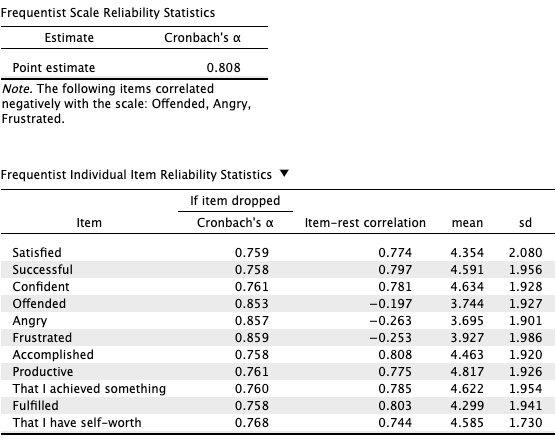
\includegraphics[width=88mm,scale=1]{Frequentist Individual Item Reliability Statistics.png}}
		\caption{Frequentist individual item reliability statistics}
		\label{Frequentist individual item reliability statistics}
		\end{figure}
	
		\subsection[htbp]{Comparing well-being and positive feedback}
		The Independent Samples T-Test examines the two sample means to see if the population means differ significantly from the sample means. It is a statistical technique used to analyze the mean comparison of two independent groups. The Independent T-Test is also called the two-sample T-Test or Student’s T-Test. 
		We used Mann-Whitney U Test as the data were not normalised.\\
		
		\begin{figure}[htbp]
		\centerline{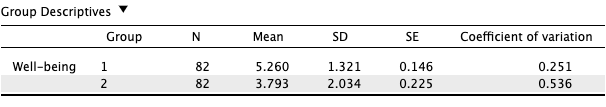
\includegraphics[width=88mm,scale=1]{Group Descriptives.png}}
		\caption{Group Descriptives}
		\label{Group Descriptives}
		\end{figure}
	
		\figurename{\ref{Group Descriptives}} indicates that the mean for Group-1 (Positive) is 5.260 and for Group 2 (Negative) it is 3.793.\\
		
		\begin{figure}[htbp]
		\centerline{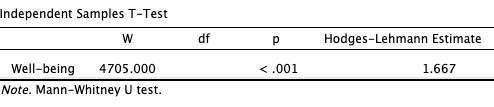
\includegraphics[width=88mm,scale=1]{Independent Samples T-Test.png}}
		\caption{Independent Samples T-Test}
		\label{Independent Samples T-Test}
		\end{figure}
	
		\figurename{\ref{Independent Samples T-Test}} shows that the $p$-value for the Independent Samples T-Test is less than the standard significance level of 0.05, we can reject the null hypothesis. The null must be removed if the $p$-value is low. Our sample data support the alternative hypothesis that positive feedback is associated with well-being. Specifically, Group 1’s mean is greater than Group 2’s mean.
	
		\subsection[H]{Comparing individual variables}
		To further study the correlation between three well-being variables and valence, we tested Spearman's Correlation. The strength of a linear link between two variables is measured by Spearman's Correlation rho. It has a value between -1 and 1, with -1 indicating a strong negative correlation and +1 indicating a strong positive correlation \cite{b18}.\\
		
		\begin{figure}[H]
		\centerline{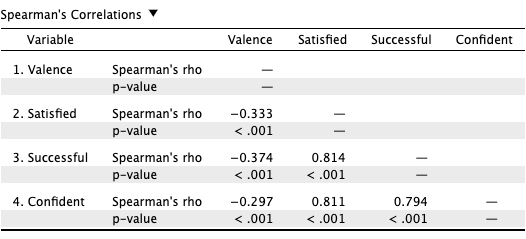
\includegraphics[width=88mm,scale=1]{Spearman's Correlations.png}}
		\caption{Spearman's Correlations}
		\label{Spearman's Correlations}
		\end{figure}
	
		\figurename{\ref{Spearman's Correlations}} shows that Spearman's Correlation rho for well-being variables responsible for positive affect lies in the range of -0.5 to 0. Hence, a strong correlation between valence and well-being parameters is proved. Considering the $p$-value, there is a significant difference between valence and well-being variables. However, well-being and valence are negatively correlated, as valence increases well-being decreases and vice versa.
	
	
\section[H]{Results}
	In this paper, the association between positive feedback and well-being was studied. More specifically, whether or not there is a relationship between valence and well-being, and whether or not well-being decreases or increases with valence change. In the analysis, after data filtration, out of 468 responses, only 164 samples were considered for further analysis. To check data reliability, a unidimensional reliability test was performed. It resulted in Cronbach’s $\alpha$ ranging from 70\% to 95\%, which is reliable, and it was verified by inspecting the mean and standard deviation. An Independent Sample T-Test was conducted on well-being as a dependent variable and valence as a grouping variable. This test resulted in a $p$-value below the standard significance level of 5\% (i.e., 0.05). Hence, the null hypothesis was rejected. Spearman's Correlation rho was used to back up this claim and investigate individual well-being variables that are responsible for positive affect, and it revealed a significant correlation between the valence and all variables. The relationship is represented using bar plot (\figurename{\ref{Bar Plot}).\\
		
	\begin{figure}[H]
	\centerline{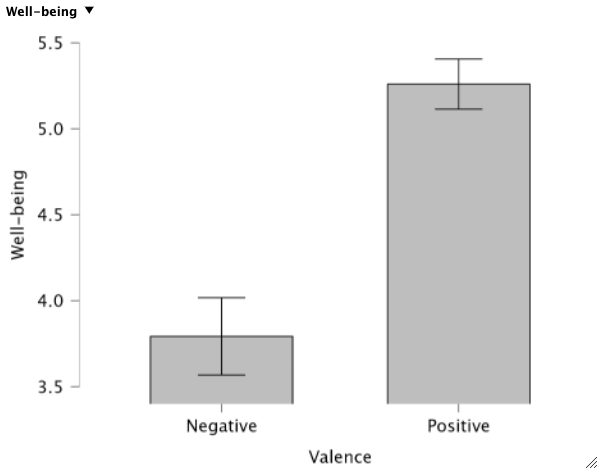
\includegraphics[width=88mm,scale=1]{Bar Plot.png}}
	\caption{Bar Plot Well-being vs Valence}
	\label{Bar Plot}
	\end{figure}
	
	After analysing all test findings, it can be said that positive feedback and well-being are correlated, and that well-being increases as the amount of positive feedback drops. 

\section{Discussion}
	The primary goal of this study was to determine the corellation between employee well-being and positive task feedback (valence) while working with intelligent assistant in manufacturing domain. Prior research has demonstrated the significance of workplace well-being for both employers and employees\cite{b7}. The study is evidence that positive task feedback contributes to well-being in the manufacturing sector and that well-being rises as positive feedback decreases.\\
	This work can be used as a reference point for fresh idea development and innovation, particularly in the area of feedback systems. The modern manufacturing sector benefits from an improvement in well-being by taking into account the dimension of positive task feedback and appreciating its value. The usage of task feedback in the manufacturing sector could be enhanced or increased with further study on this subject.\\
	The study was limited to the analysis of 164 samples and focused on positive feedback from the Affect and Authentic Pride part of well-being characteristics.
	
\section*{Acknowledgement}
	I sincerely appreciate the help and guidance received from Dr.-Ing. Dr. phil. Dr. rer. soc. Carsten Roöcker. I would especially want to thank Hitesh Dhiman, M.Sc., for his continued assistance whenever it was required, and I would also like to express my sincere gratitude to all survey respondents who gave me the insightful feedback.


\begin{thebibliography}{00}

	\bibitem{b1} Elpidio Nara, Matheus Costa, Ismael Cristofer Baierle, Lisianne Benitez
	Expected Impact of Industry 4.0 Technologies on Sustainable Development: A study in the context of Brazil's Plastic Industry.
	\bibitem{b2}A. Rojko
	Industry 4.0 concept: background and overview
	\bibitem{b3}W. Karwowski
	A review of human factors challenges of complex adaptive systems: discovering and understanding chaos in human performance.
	\bibitem{b4}C.E. Siemeniuch, M.A. Sinclair, M.J.deC. Henshaw
	Global drivers, sustainable manufacturing and systems ergonomics
	\bibitem{b5}P.W. Neumann, S. Winkelhaus, E.H. Grosse, C.H. Glock
	Industry 4.0 and the human factor – a systems framework and analysis methodology for successful development
	\bibitem{b6}Arthur A. Stonea,1, Joseph E. Schwartza,b, Joan E. Brodericka, and Angus Deaton
	A snapshot of the age distribution of psychologicalwell-being in the United States.
	\bibitem{b7}Tamao Matsui and Akinori Okada
	Mechanism of Feedback Affecting Task Performance
	\bibitem{b8}E.A. Locke, N. Cartledge, C.S. Knerr
	Studies of the relationship between satisfaction, goals setting, and performance
	\bibitem{b19}E. Pagán-Castaño, A. Maseda-Moreno, C. Santos-Rojo,
	Wellbeing in work environments
	\bibitem{b20}Jennifer L. Sparr \& Sabine Sonnentag
	Fairness perceptions of supervisor feedback, LMX, and employee well-being at work
	\bibitem{b21}Hamzah, H., Nordin, N. S., Dwiyanti, R., Na’imah, T., \& Mawi, N. 
	The Role of Well-Being, Supervisor Support and Positive Feedback on Lecturers’ Work Engagement
	\bibitem{b22}Juniper, Bridget
	Defining employee wellbeing
	\bibitem{b24}Wallston, B. S., Alagna, S. W., DeVellis, B. M., \& DeVellis, R. F.
	Social support and physical health
	\bibitem{b25}Boorse, C.
	What a theory of mental health should be.
	\bibitem{b23}Boud, D. and Molloy, E.
	What is the problem with feedback?
	\bibitem{b9}Chia-Chien Hsu \& Brian A. Sandford
	Instrumentation Pertaining to the Whole Process of Data Collection
	\bibitem{b10}JASP Team, 2022
	JASP (Version 0.16.4)[Computer software]
	\bibitem{b11}Armor, D. J.
	Theta reliability and factor scaling. Sociological Methodology, 5, 17-50.
	\bibitem{b12}Ebel, R. L.
	Estimation of the reliability of ratings. Psychometrika, 16(4), 407-424.
	\bibitem{b13}Tavakol, M. and Dennick, R.
	Making sense of Cronbach's alpha. International journal of medical education, 2, p.53.
	\bibitem{b14}Lavrakas, P.
	Encyclopedia of Survey Research Methods 1st Edition. SAGE.
	\bibitem{b15}Salkind, N.
	Encyclopedia of Measurement and Statistics 1st Edition. SAGE.
	\bibitem{b16}Nunnally J, Bernstein L.
	Psychometric theory. New York: McGraw-Hill Higher, INC; 1994.
	\bibitem{b17} Bland J, Altman D.
	Statistics notes: Cronbach's alpha. 
	\bibitem{b18}David Nettleton
	Selection of Variables and Factor Derivation

\end{thebibliography}


\end{document}
